\documentclass[10pt]{beamer}

\usetheme{Frankfurt}
\useoutertheme{default}
\setbeamertemplate{footline}[page number]
\setbeamertemplate{navigation symbols}{} 

\usepackage{cmap}					% поиск в PDF
\usepackage[T2A]{fontenc}			% кодировка
\usepackage[utf8]{inputenc}			% кодировка исходного текста
\usepackage[english,russian]{babel}	% локализация и переносы
\usepackage{indentfirst}
\frenchspacing

\newcommand{\delayV}[1]{\overset{\leftarrow}{\textbf{x}}_{#1}}

\theoremstyle{definition}
\newtheorem*{Def}{Определение}

\title{Классификация временных рядов в пространстве модели c подходом NeuralODE}
\author{Сёмкин Кирилл}

\institute[MIPT]{Московский физико-технический институт \\ Кафедра интеллектуальных систем}

\date[2024]{\textit{Научный руководитель}: д.ф.-м.н. Стрижов Вадим Викторович \\ 2024}

\begin{document}
	
	\begin{frame}[c]
		\titlepage
	\end{frame}
	
	\begin{frame}{Проблематика работы}
		
		\begin{alertblock}{Проблема}
			Необходим метод классификации временных рядов, порождаемых скрытыми динамическими системами. Классификация без учёта порождения данных может быть неустойчивой и некорректной.
		\end{alertblock}
		
		\begin{block}{Цель}
			Ввести вероятностную постановку порождения временных рядов в связке с моделью \emph{ОДУ}. Решить проблему ненаблюдаемости порождающих динамических систем. Сформулировать формальную задачу классификации и предложить способы решения.
		\end{block}
		
		\begin{exampleblock}{Решение}
			% Использовать \emph{теорему Такенса} для восстановления зашумлённых фазовых траекторий,
			Использовать \emph{NeuralODE} для аппроксимации динамических систем. Параметры системы могут быть фиксированными или порождаться \emph{априорным} распределением. Классификацию осуществлять с помощью \emph{байесовского тестирования гипотез} или строить классификатор в пространстве параметров дин. системы.
		\end{exampleblock}
		
	\end{frame}	
	
	\begin{frame}{Постановка задачи}
		
		Задана обучающая и тестовая выборка временных рядов для каждого класса. Количество классов $K$.
		
		Пусть для каждого класса существует динамическая система $\textbf{f}_i$, порождающая траектории $\textbf{z}(t)$ что
		
		\begin{equation*}
			\begin{cases}
				\dfrac{d \textbf{z}}{dt} (t) = \textbf{f}_i \big( \textbf{z}(t) \big), \\
				\textbf{z}(0) = 0.
			\end{cases}
		\end{equation*}
		
		Пусть существует \emph{функция наблюдений} $\phi$: $\phi\big( \textbf{z}(t) \big) = x(t)$.
		
		\begin{figure}
			\centering
			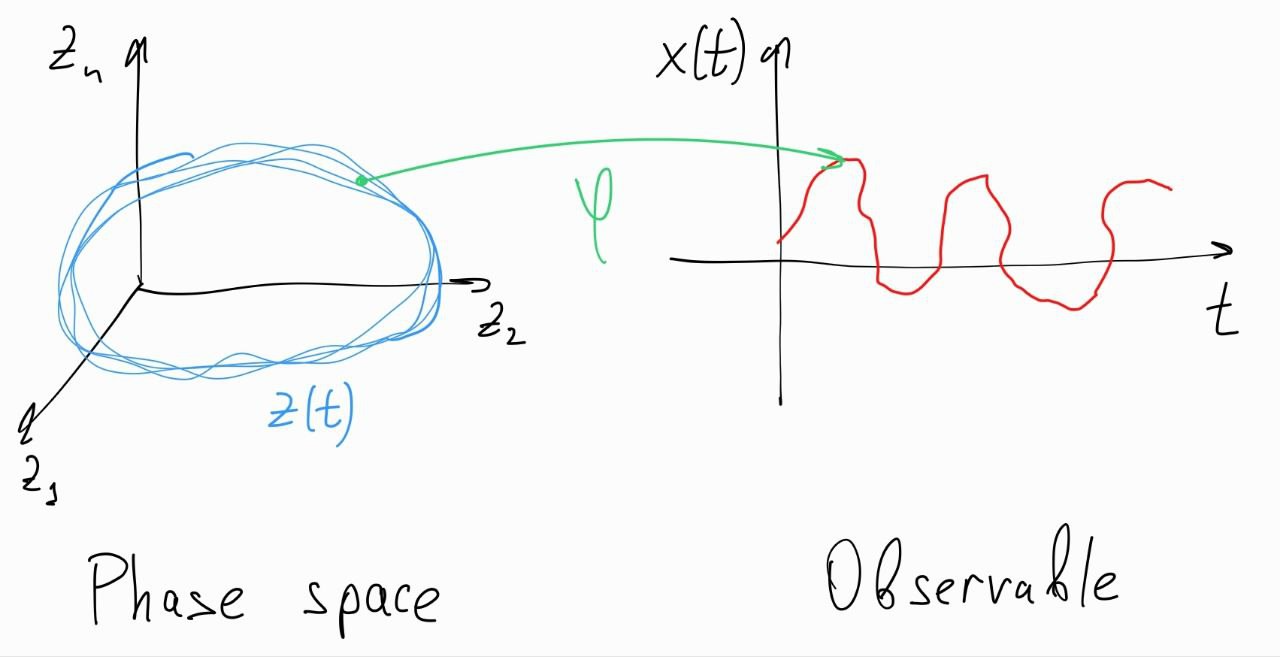
\includegraphics[width=0.7\textwidth,keepaspectratio]{img/phi_func.png}
		\end{figure}
		
	\end{frame}	
	
	\begin{frame}{Восстановление и параметризация дин. системы}
		
		Наложив некоторые условия регулярности на $\textbf{f}_i$ и $\phi$, с помощью теоремы Такенса можем получить \emph{вложение} исходных дин. систем в $\mathbb{R}^m$. Фазовыми траекториями будут \emph{вектора задержки} $\delayV{t}$
		
		\begin{equation*}
			\textbf{z}(t) = \delayV{t} := \begin{pmatrix}
				x(t - L + 1) \\
				\vdots \\
				x(t - 1) \\
				x(t)
			\end{pmatrix} \in \mathbb{R}^m.
		\end{equation*}
		
		Предположим, что векторные поля $\textbf{f}_i$ лежат в известном параметрическом классе, т.е. $\textbf{f}_i = \textbf{f}_{\Theta_i}$. Наконец наложим на тректории независимый шум с нулевым средним и ограниченной дисперсией
		
		\begin{gather*}
			\textbf{z}(t) \to \textbf{z}(t) + \boldsymbol{\epsilon}, \\
			\text{s.t. } \mathbb{E}[\boldsymbol{\epsilon}] = 0, \, \mathbb{D}[\boldsymbol{\epsilon}] < +\infty.
		\end{gather*}
		
	\end{frame}	
	
	\begin{frame}{Полная модель порождения данных}
		
		Предлагаются три типа связи параметров $\Theta_i$ с дин. системами $\textbf{f}_i$ в рамках класса:
		
		\begin{enumerate}
			\item Дин. система класса имеет фиксированные параметры $\Theta_i = $ const. 
			
			\item Класс имеет \emph{априорное} распределение на параметры $\Theta_i \sim p_i(\Theta)$ (генеративная модель).
		\end{enumerate}
		
		Добавив априорное распределение на классы $ C \sim \text{Cat}(C) $, мы полностью определим вероятностную модель задачи.
		
		\begin{enumerate}
			\setcounter{enumi}{2}
			\item Каждый параметр $\Theta$ задаёт распределение на класс $C \sim p(C | \Theta)$ (дискриминативная модель).
		\end{enumerate}
		
		\begin{figure}
			\centering
			%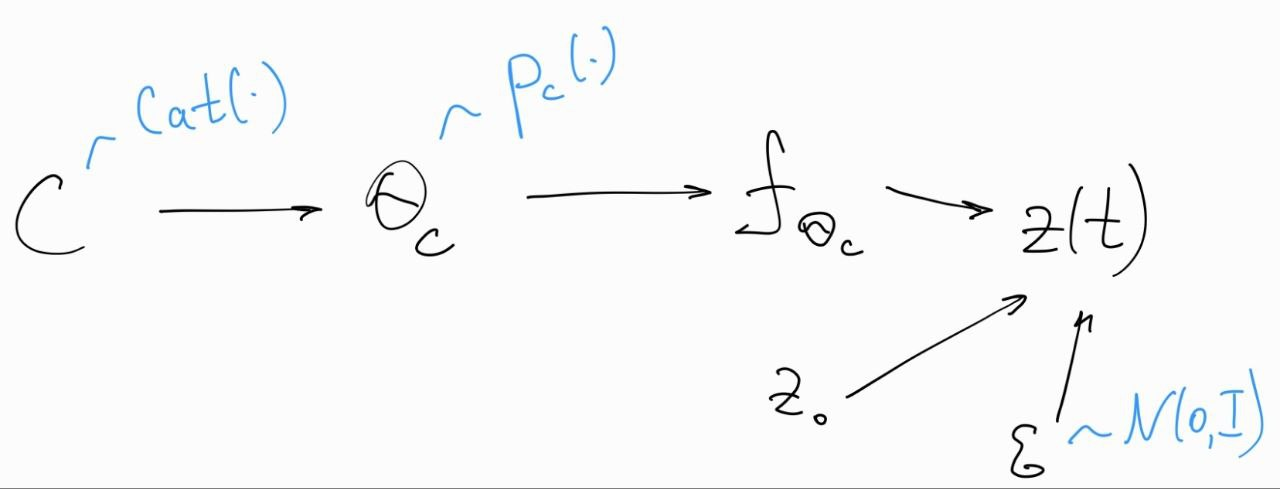
\includegraphics[width=0.7\textwidth,keepaspectratio]{img/bayes_graph_gen.jpg}
			%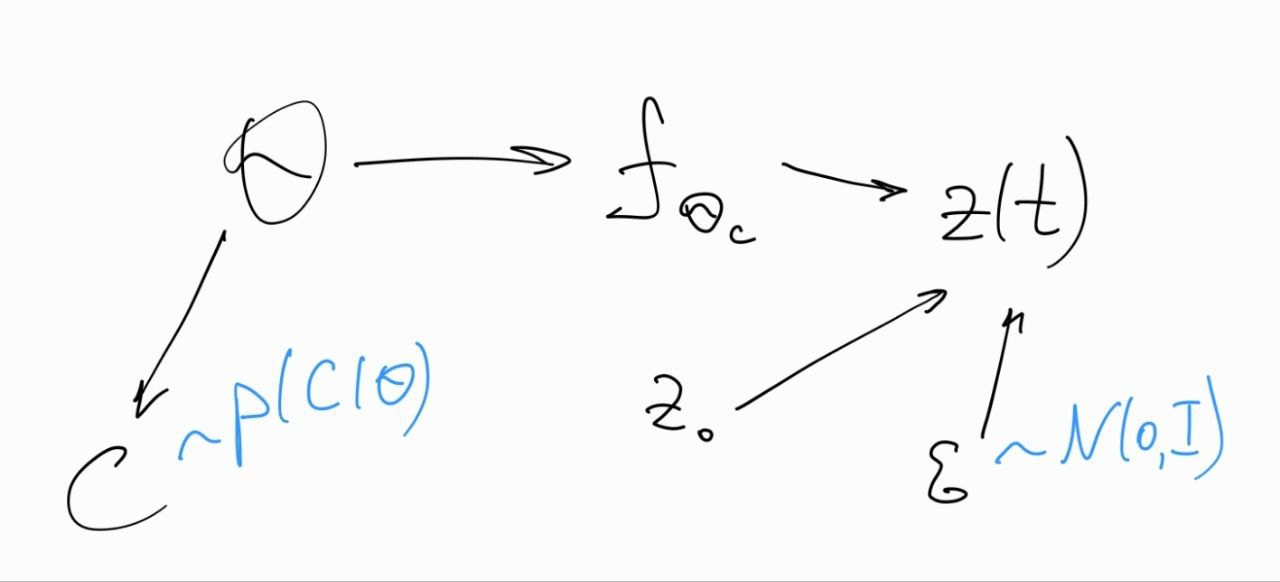
\includegraphics[width=0.7\textwidth,keepaspectratio]{img/bayes_graph_discr.jpg}
		\end{figure}
		
	\end{frame}

	\begin{frame}{Алгоритмы классификации временных рядов}
		
		Для каждого типа связи:
		
		\begin{enumerate}
			\item На обучающей выборке получить ML оценки параметров класса $\hat{\Theta}_i$. Для тестовой траектории воспользоваться \emph{байесовским решающим правилом}:
			
			\begin{equation*}
				C_{\text{test}} = \underset{C_i}{\arg \max} \, p(C_i) p\big( \textbf{z}_{\text{test}}(t) | \hat{\Theta}_i \big)
			\end{equation*} 	
			
			\item Байесовский вывод
			
			\begin{equation*}
				p \big(C = C_i | \textbf{z}_{\text{test}}(t), \textbf{z}_{\text{train}}(t) \big) = \int p \big( C = C_i | \Theta, \textbf{z}_{\text{test}}(t) \big) p_i \big( \Theta | \textbf{z}_{\text{train}}(t) \big) d\Theta
			\end{equation*}
			
			\item По каждой обучающей траектории получить ML оценку порождающей дин.системы $\hat{\Theta}$. Далее, на полученных оценках обучить классификатор в пространстве параметров $p(C | \Theta)$. Для тестовой траектории снова получаем оценку $\hat{\Theta}_{\text{test}}$, пользуемся классификатором:
			
			\begin{equation*}
				C_{\text{test}} = \underset{C_i}{\arg \max} \, p(C_i | \hat{\Theta}_{\text{test}})
			\end{equation*}
		\end{enumerate}
		
	\end{frame}	
	
	\begin{frame}{Постановка эксперимента}
		
		\begin{block}{Цель эксперимента}
			Восстановить фазовые траектории и скрытые дин. системы по обучающей выборке, сравнить качество классификации тремя предложенными методами + c моделями RNN, CNN. Оценить применимость предложенных методов.
		\end{block}
		
		\begin{exampleblock}{Данные}
			Акселерометрия движений человека для разных типов активностей (50 Гц, 6 классов), датасет \href{https://github.com/mmalekzadeh/motion-sense}{MotionSense}.
		\end{exampleblock}
		
		\begin{figure}[h]
			\centering
			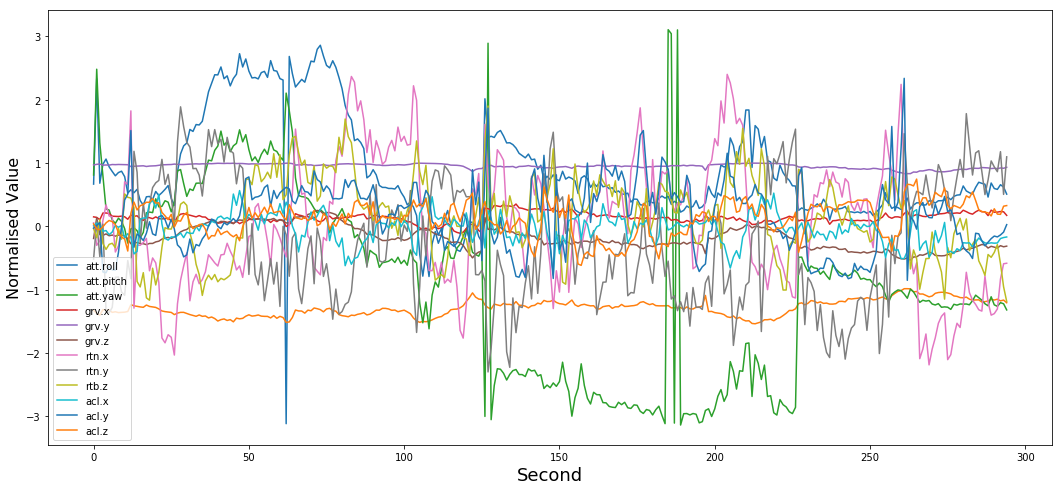
\includegraphics[width=0.6\textwidth]{img/motionsense}
		\end{figure}
		
	\end{frame}	
	
	\begin{frame}{Фазовые траектории}
		
		Временные ряды активности "upstairs" и восстановленные фазовые траектории.
		
		\begin{figure}
			\centering
			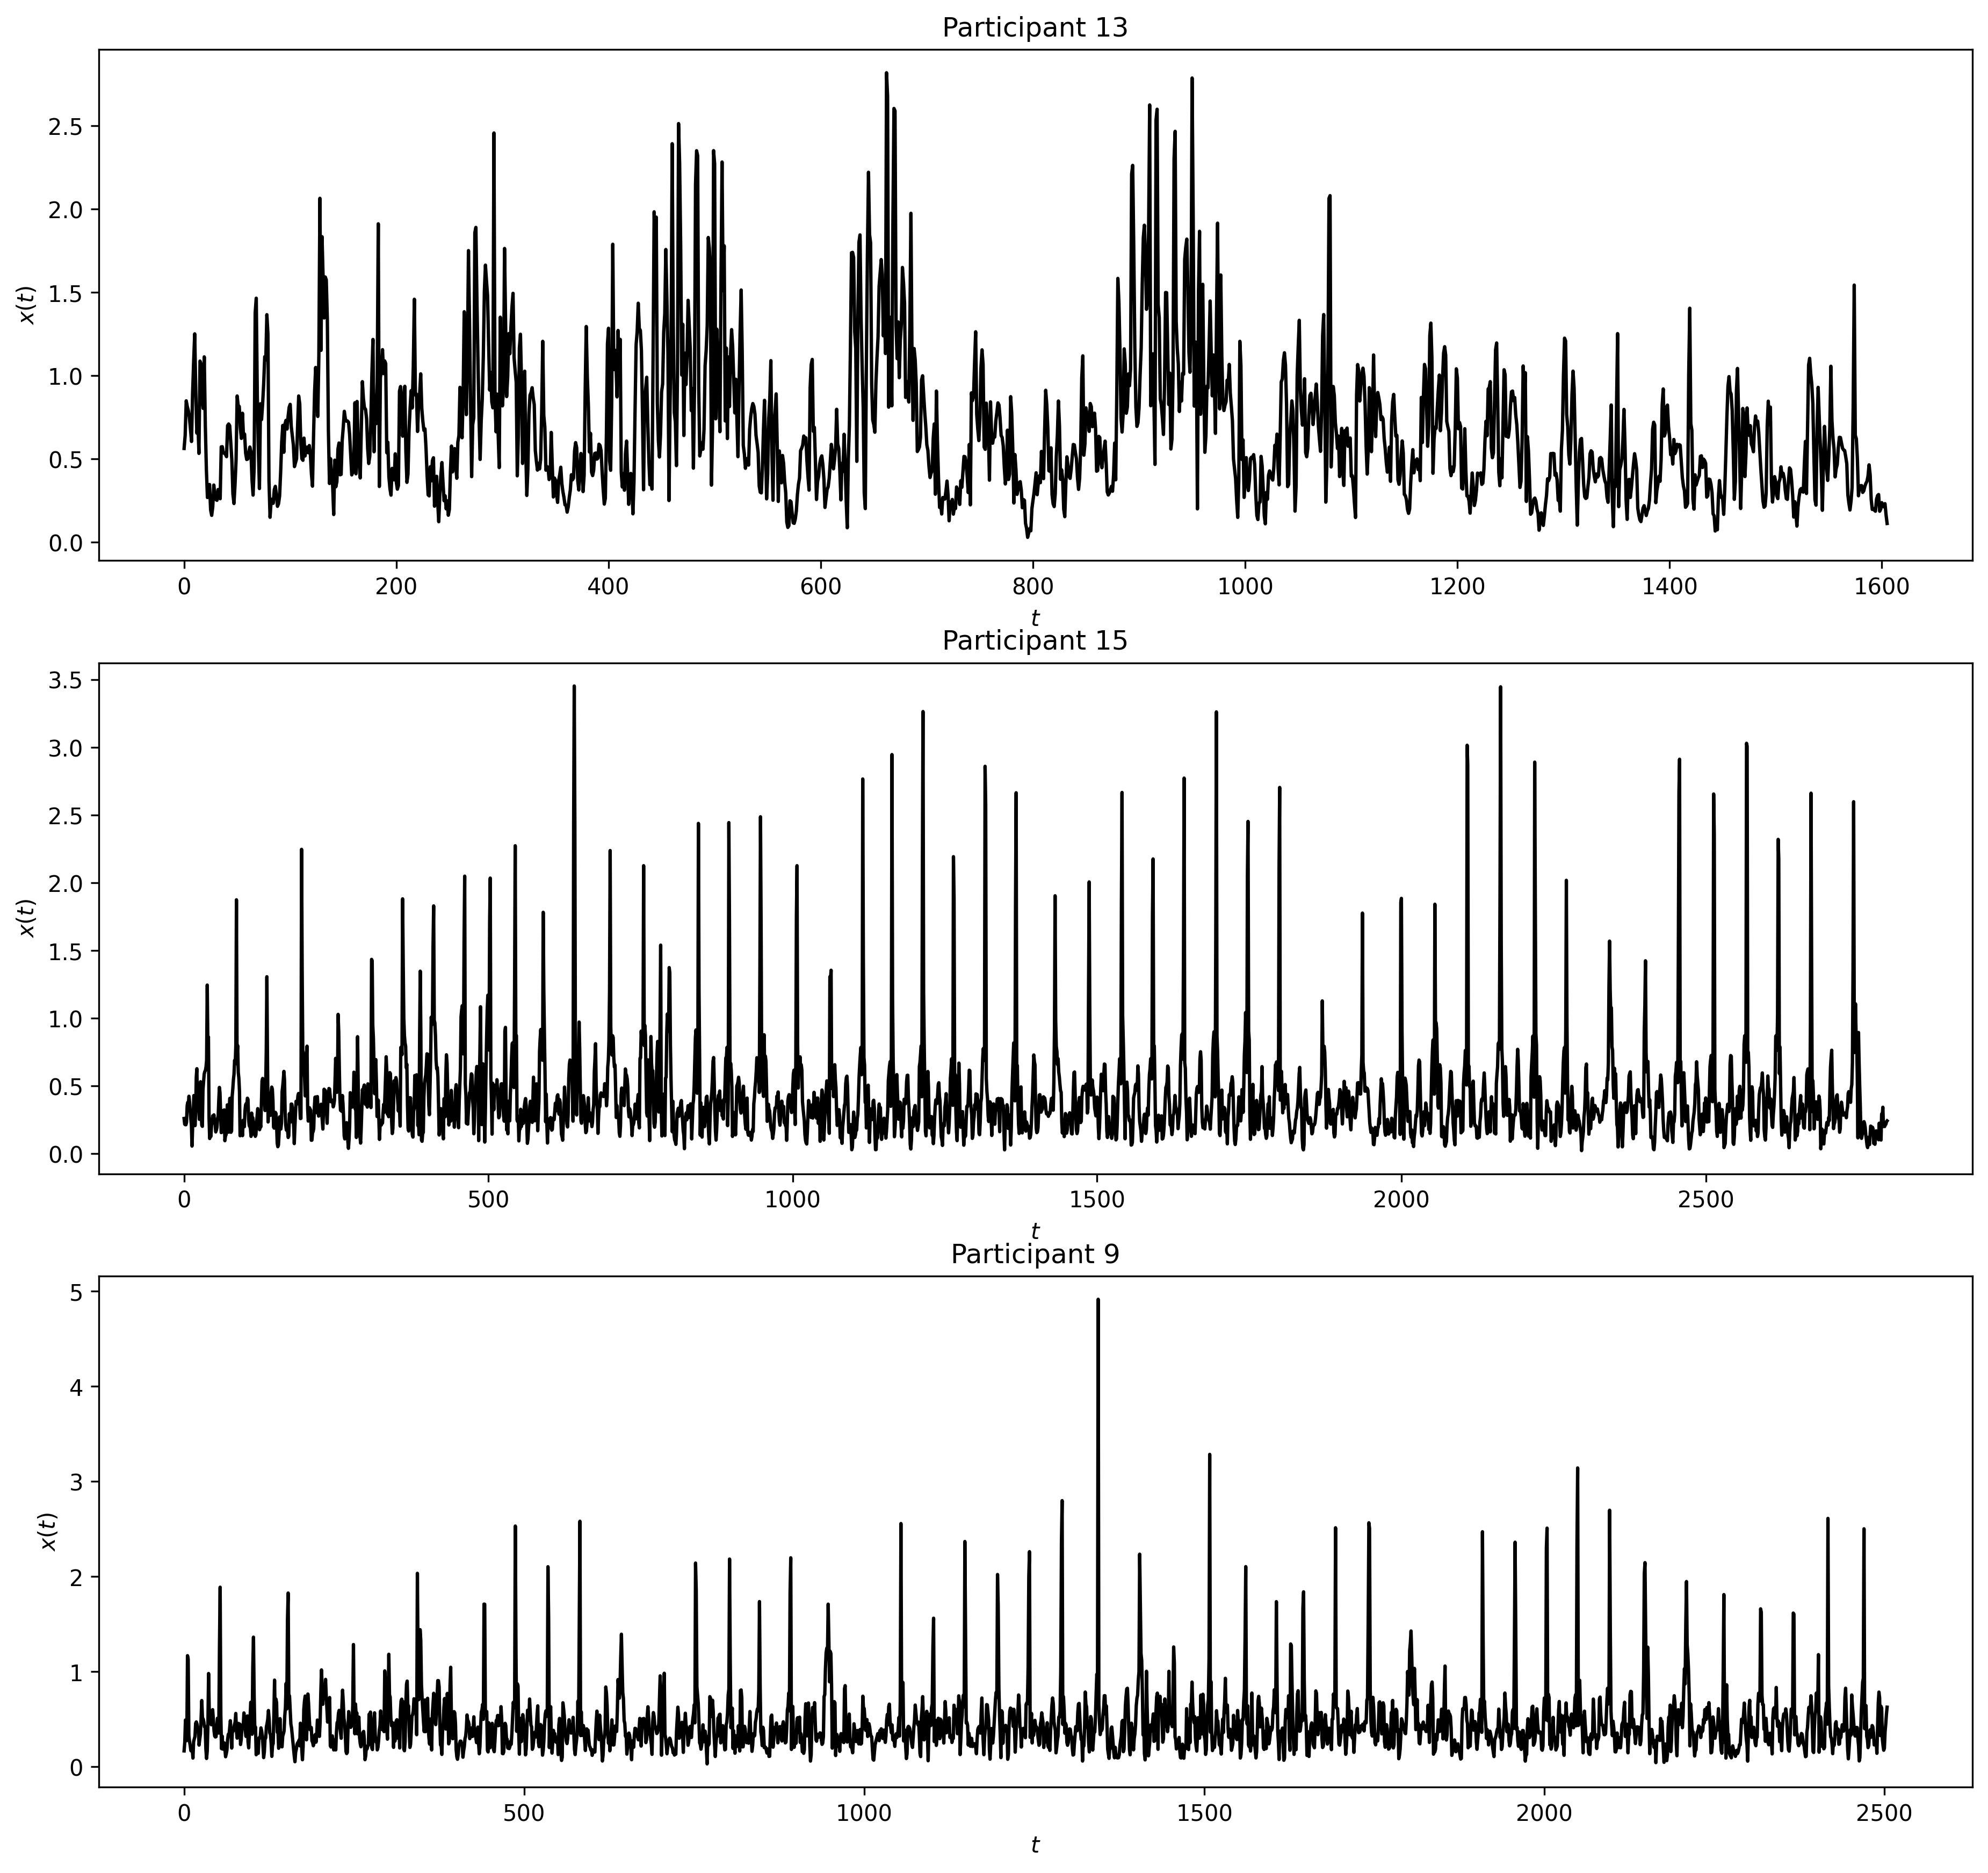
\includegraphics[width=0.4\textwidth]{img/series_ups.png}
			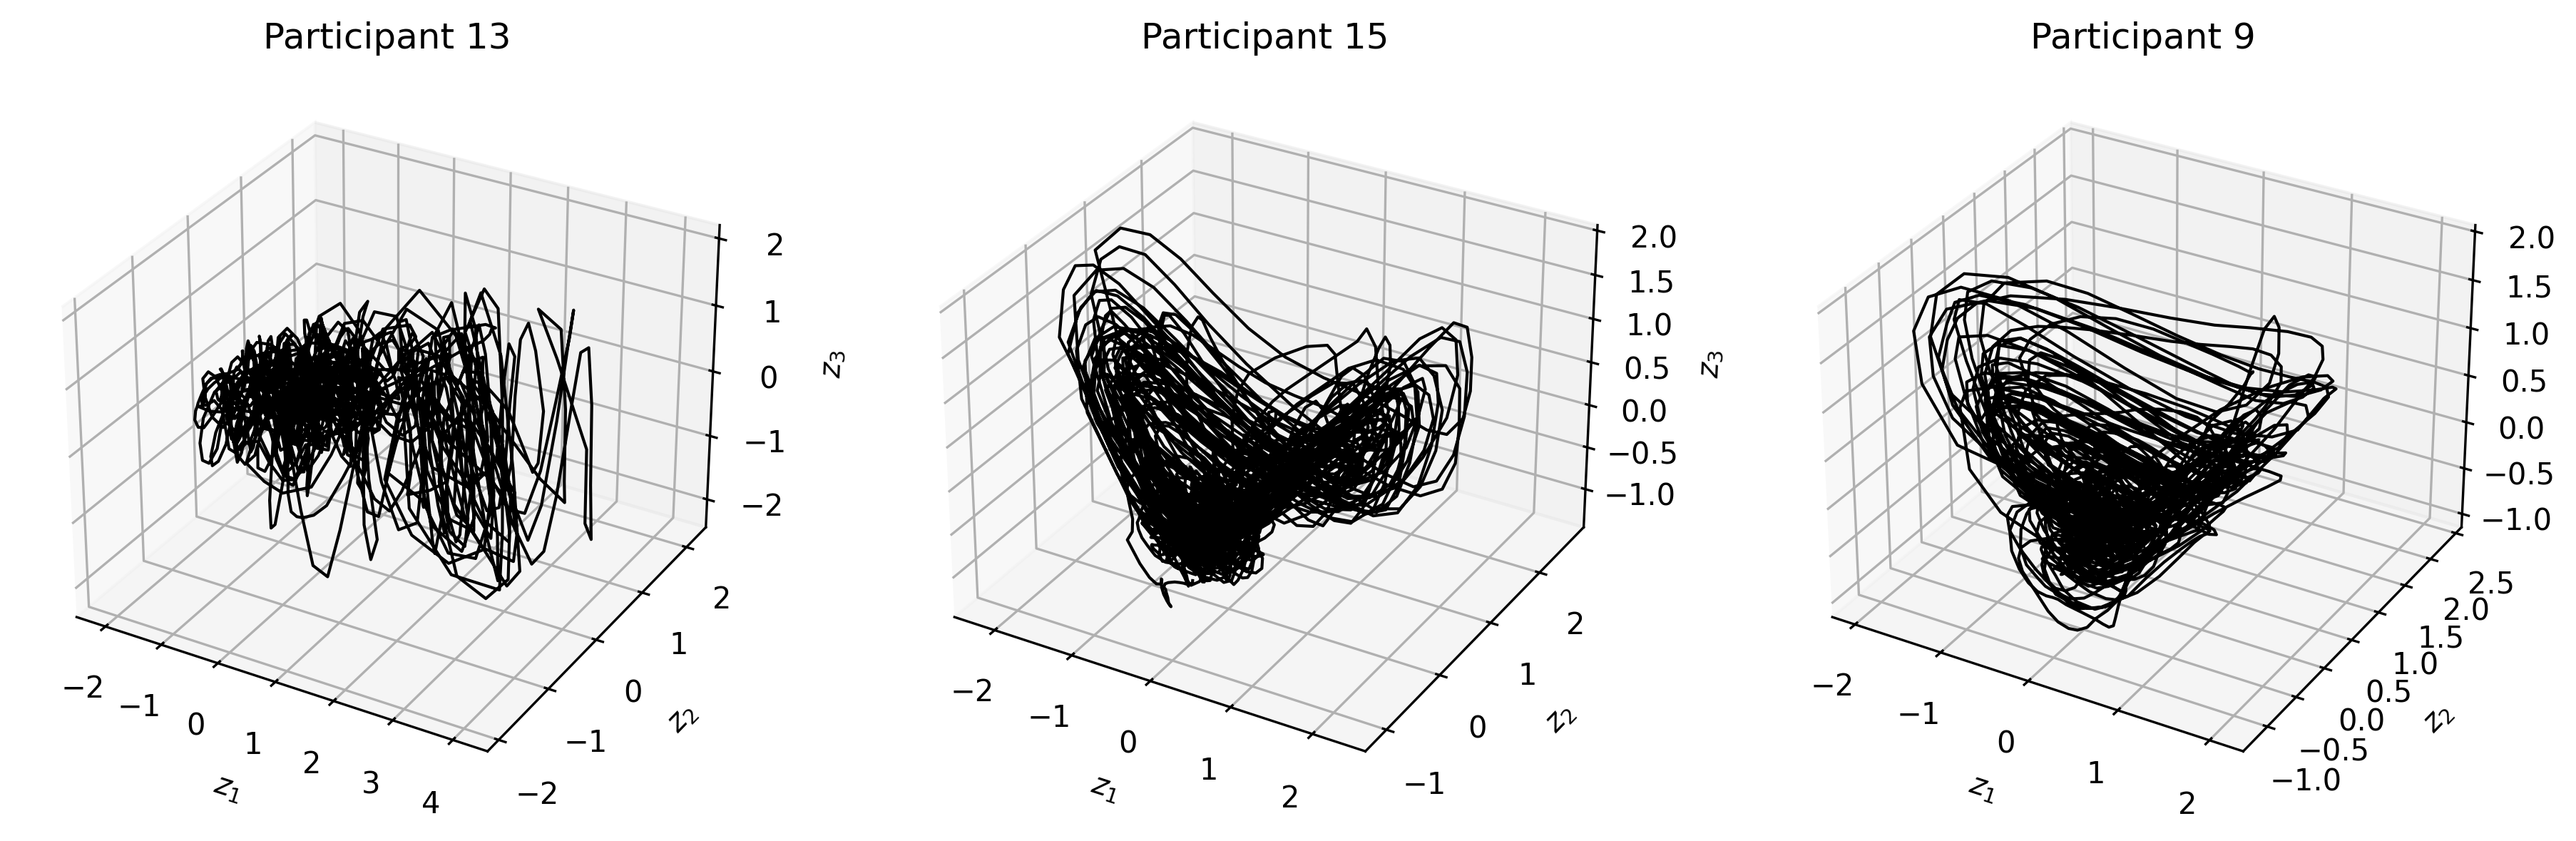
\includegraphics[width=0.59\textwidth]{img/phase_ups.png}
		\end{figure}
		
	\end{frame}	
	
	\begin{frame}{Байесовское решающее правило}
		
		
		
	\end{frame}	
	
	\begin{frame}{Классификация в пространстве параметров}
		
		
	\end{frame}	
	
\end{document}